%*******************************************************************************
%****************************** Fifth Chapter *********************************
%*******************************************************************************

\chapter{Methodology}

\ifpdf
    \graphicspath{{Chapter5/Figs/Raster/}{Chapter5/Figs/PDF/}{Chapter5/Figs/}}
\else
    \graphicspath{{Chapter5/Figs/Vector/}{Chapter5/Figs/}}
\fi

%********************************** %First Section  **************************************
\section{Definitions and assumptions}

We make the following definitions:
\begin{enumerate}
\item A "channel" refers to image data gathered via a particular method of detection. Brightfield data is one channel. GFP fluorescence data is another channel. Two channels can gather data on a single physical area or volume. However, each channel records and stores data separately.
\item A "frame" refers to a particular point in time at which a channel produces an image. It should be noted that in reality an image is not produced instantaneously, and thus a frame actually refers to a relatively short period of time.
\item A "pixel" refers to a data structure that holds an intensity value. This value represents the intensity of light (visible or fluorescent) detected on a square section of a physical detector during the set exposure time period.
\item "x" and "y" are the x-coordinate and y-coordinate of a pixel within a single image.
\item A "stack" refers to the image set produced by a confocal microscope at a particular frame. A stack can be visualised as a collection of images positioned vertically on top of each other, aligned in x and y such that a pixel's x-y location in a particular image is directly underneath or above its equivalent in any other image.
\item All images in a stack are considered to be produced at the same frame.
\item "z" is the index of an image within a stack. It can be thought of as the image's "height" or "level" within a stack. We use the term "z-value" to mean the height (e.g. of a pixel) in the z-dimension of the stack.
\item "pixel value" refers to the intensity value at a particular pixel in a specific image.
\item A "profile" is the distribution of intensity values obtained by taking a fixed x-y location and steadily incrementing z over the entire stack, noting each intensity value at each level. It should be noted that the fixed location could be a 2D array (in x and y) of pixels, not just a single pixel. Generally, however, we use the term "profile" in this paper to mean the profile of a single pixel x-y location through the whole stack.
\item A "cell pixel" refers to a pixel that, at a particular frame, is considered (by a human or by an algorithm) to represent a component section of a cell. The cells move and change shape, so that a given pixel may only be a cell pixel during a few frames.
\item A "cell instance" is the data object that contains a group of cell pixels that comprise one particular cell at a particular frame.
\end{enumerate}

\begin{figure}[htbp!]
\centering
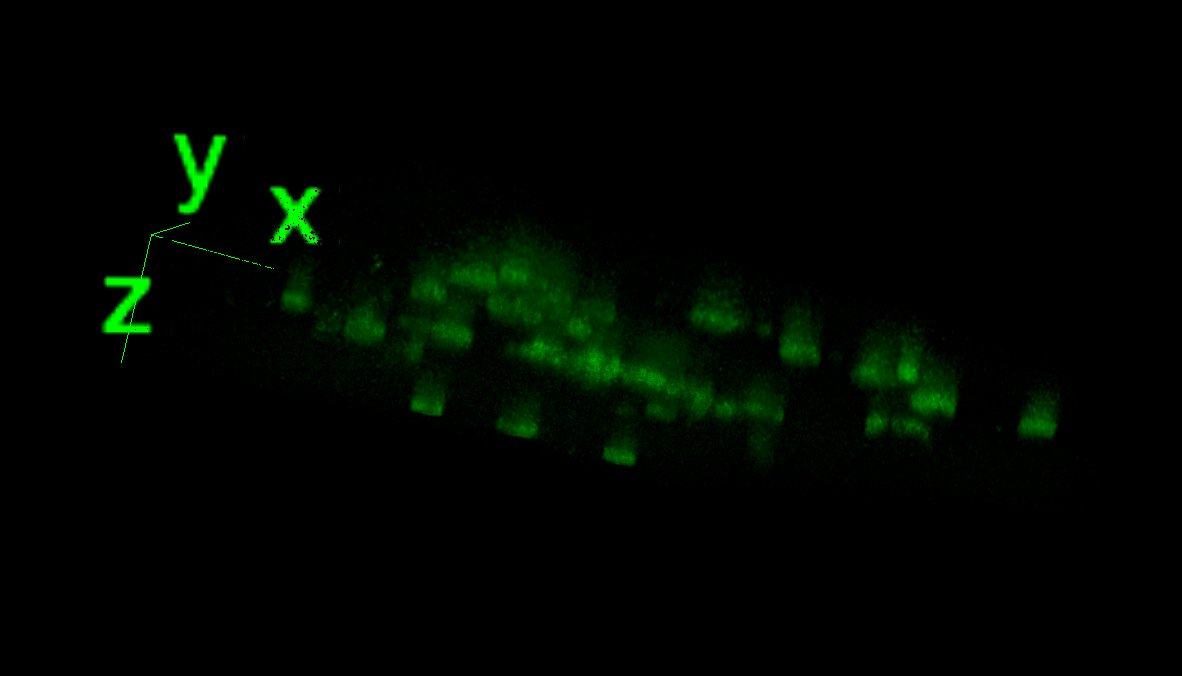
\includegraphics[width=1.0\textwidth]{3D_gfp_extended_tails}
\caption[GFP 3D reconstruction]{Extended regions of GFP intensity can be seen trailing from otherwise normal lenticular reconstructions of cells in 3D.}
\label{fig:gfp_3d_recon}
\end{figure}

In addition, some assumptions are made about the environment and the imaging process:
\begin{enumerate}
\item In this 3D reconstruction of the GFP, cells are shown as flat discs in the z-dimension. Unfortunately, they are surrounded by high levels of noise, shown in Figure~\ref{fig:gfp_3d_recon}. We can't trust the GFP to produce an accurate 3D reconstruction of the cells, but we assume that the vertical position in z of maximum GFP intensity corresponds with the z-location of the cell in reality.
\item We assume for our method that the 2D intensity discontinuities of the Brightfield edges can be approximated by a single function. In reality, even within a single cell, the functional form of the edge discontinuity can change significantly.
\end{enumerate}

\section{GFP profile}

\begin{figure}[htbp!]
\centering
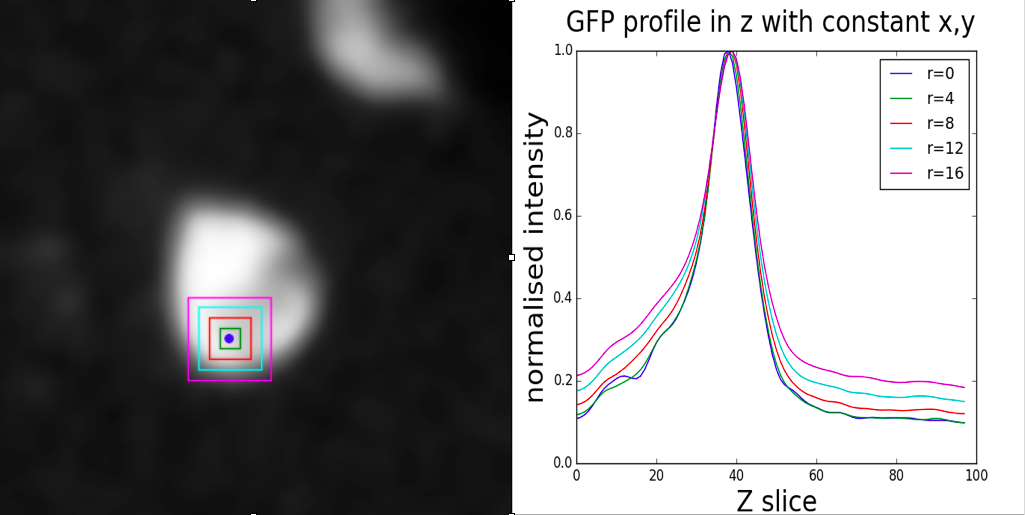
\includegraphics[width=1.0\textwidth]{411-profile}
\caption[GFP profile]{The 3D GFP profile.}
\label{fig:3D_gfp_profile}
\end{figure}

In our experimental setup, the cells have very high fluorescence intensity compared to the background environment. Using the data from the GFP channel, we create a profile for each pixel. This GFP pixel profile is the basis for our combination algorithm. An example for a single pixel is shown in Figure~\ref{fig:3D_gfp_profile}

If the profile does not pass through a cell, it will be comprised only of GFP background noise. The distribution of its values will have low variance and be quite flat. Conversely, over a z-range where a GFP pixel profile passes through a cell instance, the profile will contain very high intensity values. The distribution will have high variance and a peak will be visible. In general, the description of a pixel profile that intercepts a cell is as follows: It will start at a low value where the cell is not present, slowly increase to a maximum at the centre of the cell in the z-dimension, and decrease again on the other side of the cell. If a profile passes through the edge of a cell, it will still show a peak, but the peak will be smaller and less distinct. These types of peak can be compared in Figure~\ref{fig:gfp_profile_scatter}.

We investigated three properties of the profile intensity distributions in particular: The mean, the variance, and the z-location of the profile peak.

\begin{figure}[htbp!]
\centering
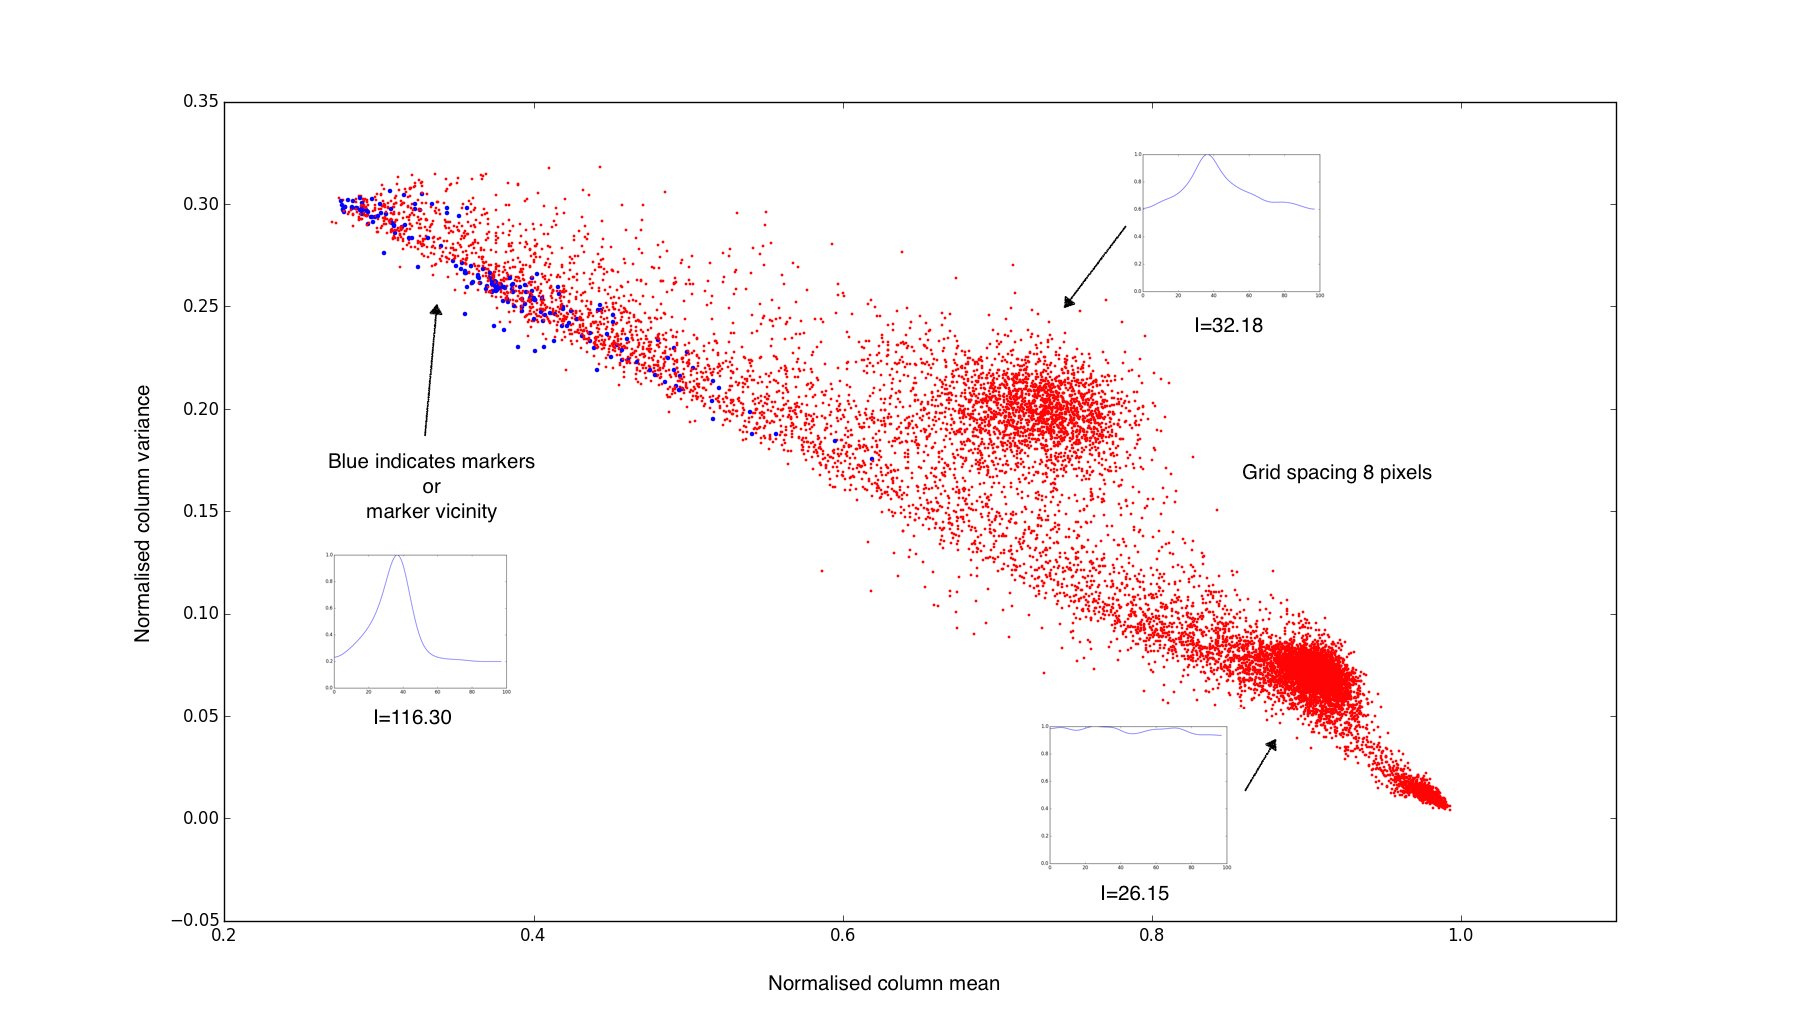
\includegraphics[width=1.0\textwidth]{412-scatter}
\caption[GFP profile types scatter plot]{A scatter plot of GFP profile mean value against the variance. Several different types of profiles can be distinguished. Profiles from the centres of cells are found in the top left with low means and high variances. Blue points represent manually chosen points. Edge profiles cluster in a large group in the centre with median mean values and median variances. Points in the background tend to have a high mean and low variance. These are normalised values, so high mean indicates a very flat distribution.}
\label{fig:gfp_profile_scatter}
\end{figure}

During examination of these profile properties, we found a fairly linear relationship between normalised mean and variance. The profile distribution data was normalised by dividing every profile value by the maximum profile value. We then plotted the normalised variance against the normalised mean. This linear relationship shows that we can parameterise one property in terms of the other, so for the rest of this method we focus on only one of the two properties; the mean.

There are three distinct observable groups in this graph. The first group has a high mean and a low variance. This indicates a profile that contains only GFP background noise. The second group has a low mean and high variance. This indicates a clear peak in the GFP profile. The third group clusters above the conceptual line of best fit, having a medium mean and medium variance. This indicates a profile that passes through the edge of a cell. It has a peak but one that is less distinct.

The blue points represent the profiles of a set of manually marked pixels from the manual tracking step. These profiles are clustered in the group of profiles of cell pixels. Their clustering demonstrates the consistency of the profile distribution groupings. We conclude that we can rely on these profile patterns to stay fairly constant during experiments. We can therefore develop image processing techniques that make use of this reliability.

\section{Generating zMod}

From each 3D GFP image stack, we produce a new 2D image that we term zMod. For each profile in the stack, we find the z-location of its intensity peak. It should be noted that for background noise profiles, the z-location of the greatest absolute value will be somewhat random. It should also be noted that the PDMS barriers and pillars show even lower levels of noise and therefore have very flat GFP profile distributions, so their intensity peaks in z will be very random. We then set each pixel value in zMod to be proportional to this peak z-location. The resulting image is analogous to a terrain map. It collates the "heights" of each GFP peak in the 3D data into a single image. Low pixel values correspond to low heights and vice versa. We represent low values as dark pixels and high values as bright pixels.

This is similar to the method used by Selinummi et al. [ref], except that the Brightfield distributions, when generated in the same way as the GFP profile, do not produce intensity peaks at relevant locations, such as the centre of the cells. Therefore, the peaks in those distributions do not necessarily correspond to the vertical position of the cell in the z-dimension. The GFP profile might vary from the background noise in the same manner as the Brightfield profile, but the GFP profile accurately determines the cell height in the 3D environment.

The focal plane that contains the most high-quality GFP results may not be the same focal plane that is best for segmenting cells. We refer to the difference in z between these two planes as "delta-z". During this project, we found the value of delta-z to be constant for a given microscope and specific experiment. Delta-z is found by manually iterating over z in a stack until the selected image shows the characteristics that are helpful for segmentation. We then add the value of delta-z to every pixel in zMod. This slightly adjusts the stack "heights" represented by the pixel values in zMod.

If the shift in stack heights is large enough, a cell pixel may be moved past the limits of the 3D environment representation. In this case, either new data must be invented to fill the areas around the cell pixel(s) or the data must be truncated. Neither solution is desirable. However, this situation has not been encountered during this project. Delta-z is usually small and the cells are rarely located at the top of the environment.

\section{Generating zBF}

We then use zMod to produce another 2D image that we term zBF (for "zBrightfield"). We iterate over the image zMod, pixel by pixel, and use each pixel value to select a z-location in the original 3D Brightfield stack. We then use the pixel intensity value at this height in the Brightfield stack as the value for this x-y location in zBF.

Essentially, we have used the GFP fluorescence data to find the best focal plane for Brightfield observation of each individual cell pixel. Cell objects may spread through more than one focal plane (depending on the resolution), so a focal plane is selected for each cell pixel individually. We then extracted the corresponding pixel values from the 3D Brightfield stack and combined them into a single 2D composite image. Ideally, each cell object should now be in focus. Cell features should now be ideal for segmentation.

\section{Manual tracking}

Tracking was performed using ImageJ manual tracking software. A user performs manual tracking by clicking on cells in a simple computer interface, frame by frame. The user tracks one specific cell at a time, proceeding through the entire time series of frames for a particular location, searching only for this cell. This is done so that the software can assign a definite numeric ID to specific cells. It is also easier for the user to track one cell from frame to frame instead of many cells simultaneously.

A user might spend 30 minutes to an hour tracking cells through a typical series produced using our experimental setup, depending on the number of cells involved. The user must judge whether a particular cell is worth tracking. If a cell is mostly obscured for the whole series, there is not point trying to track it, even though it obviously exists. The user chooses not to track a particular cell by simply not clicking on it.

We use some image processing to improve the contrast between the cells and the rest of the environment. This makes the cell locations clearer for the user and increases the speed of performing manual tracking.

From each 3D GFP image stack, we produce a new 2D image that we term zMean. We take each GFP pixel profile, normalise the intensities by dividing every value by the maximum value (the height of the GFP intensity peak), and then calculate the mean of the normalised distribution. Profiles with peaks will have low normalised means. Profiles of background noise will have high normalised means. We therefore invert the mean, so that this algorithm will produce a high value for a profile that passes through a cell and low value for one that contains only background noise. We then store this value at the corresponding pixel in zMean. The final image is shown in Figure~\ref{fig:zmean_example}

\begin{figure}[htbp!]
\centering
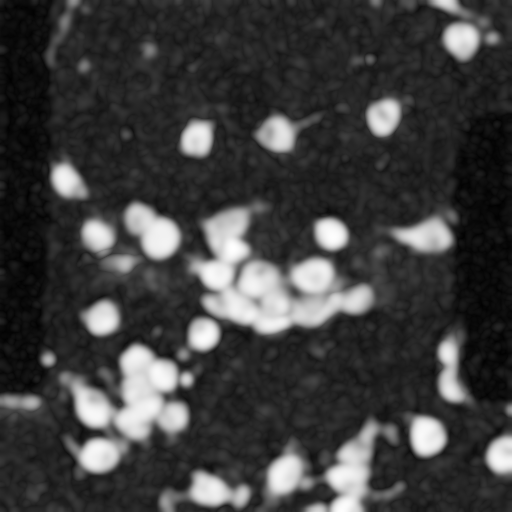
\includegraphics[width=1.0\textwidth]{zmean_example-050714_s13_ch-zmean-8-3-3_t0_z00}
\caption[zMean image example]{An example of a typical zMean image.}
\label{fig:zmean_example}
\end{figure}

We then multiply each pixel value in zBF by the corresponding pixel value in zMean. This raises the intensity of the cancer cells and darkens everything else in the image. We term the resulting image zComp, shown in Figure~\ref{fig:zcomp}.

\begin{figure}[htbp!]
\centering
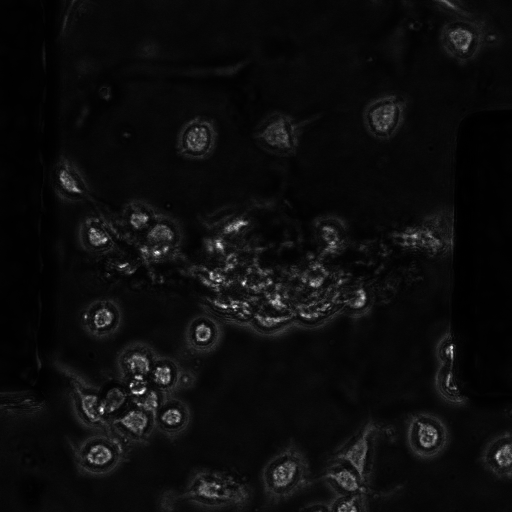
\includegraphics[width=1.0\textwidth]{431-zcomp_example-050714_s13_ch-zcomp_t00_z00}
\caption[zComp image sample]{An example of a zComp image.}
\label{fig:zcomp}
\end{figure}

Cell features such as protrusions are rather faint in raw GFP data, but in zComp the normalisation causes them to show up strongly. This highlighting effect helps a user to track cells much more quickly.

This is similar to the approach used by Selinummi et al. Because of the normalisation, the mean is statistically equivalent to the standard deviation used by Selinummi et al.

\section{Generating zEdge to prevent CellProfiler mis-recognitions}

We now use the results of the manual tracking to produce a new 2D image that we term zDiff. Each manually-chosen marker has an x-y location. We need the z-value of the marker. zMod stores the z-values of the GFP intensity peaks, so we simply take the zMod pixel value at the marker's x-y location as the marker's z-value. Then, for each marker, we produce a temporary 2D difference image by iterating over each pixel and finding the difference between its profile's GFP peak z-value and the marker's z-value. A simple subtraction will yield low values for similar heights. We then invert the result so that pixels with similar GFP peak heights to this specific marker will have high values. We threshold each temporary difference image according to full-width, half-maximum (FWHM) value of the image's z-range. We now iterate over each x-y location and choose the maximum available value from the set of difference images. We then assign this value to the pixel at that x-y location in our final 2D difference image, zDiff.

It should be noted that some background noise pixels elsewhere in the image might have GFP peaks at the same z-level as a marker. This will be included in zDiff. Hopefully, when we threshold zDiff, these background noise results will be suppressed. However, this may not happen if the noise pixels are adjacent to any of the cell pixels.

\begin{figure}[htbp!]
\centering
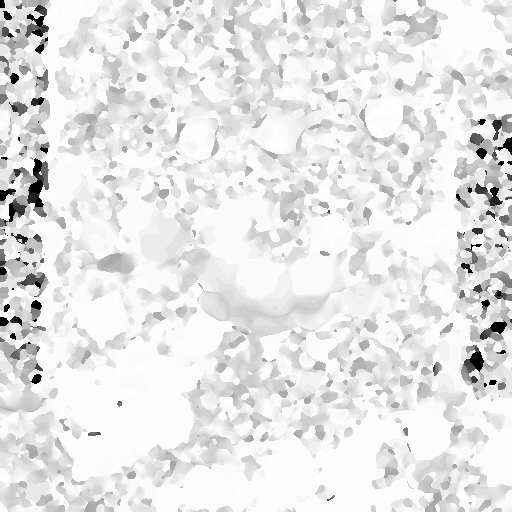
\includegraphics[width=1.0\textwidth]{zdiff_example}
\caption[zDiff image sample]{An example of a zDiff image.}
\label{fig:zdiff}
\end{figure}

zDiff is a 2D image with large, incoherent blobs that lack detail, as in Figure~\ref{fig:zdiff}. However, each blob defines the limit of relevance within an image for a particular cell, according to the GFP. We can use this to limit the effect of a CellProfiler misrecognition error. We therefore use the blob outlines of zDiff to draw artificially darkened edges onto zBF. CellProfiler misrecognitions will generally not be able to spill out beyond these strengthened edges. We term the resulting image zEdge.

\section{Sensitivity analysis of zMod parameters}

The masks found by segmentation of zEdge are compared to the masks of some ground truth. In this case, we used manual segmentation for the ground truth. This is also compared firstly to the segmentation that uses the preprocessing method of Selinummi et al. and secondly to their ground truth (the GFP projection segmentation). Selinummi et al. define formulae for precision and recall, which are then combined to give a value for the Fscore.

To compare two versions of segmentation of the same cell, one is defined as the ground truth. Observing the segmentation pixel-by-pixel, three parameters are used, true positive (TP), false positive (FP), and false negative (FN). Pixels that are true positive are contained both in the ground truth segmentation and the version of segmentation under testing. False positives are contained in the test segmentation but not in the ground truth. False negatives are contained in the ground truth but not in the test segmentation. These three parameters can be combined into two parameters, precision and recall, which are defined by the following formulas:

\begin{equation}
Precision = \frac{TP}{TP + FP}
\end{equation}

\begin{equation}
Recall = \frac{TP}{TP + FN}
\end{equation}

A perfect precision indicates that every pixel in the test also exists in the ground truth. A perfect recall indicates that every pixel in the ground truth is reproduced in the test. The reduced mean of these two parameters is termed the Fscore of the test segmentation algorithm. The Fscore is defined by the following formula:

\begin{equation}
Fscore = \frac{2 \times Precision \times Recall}{Precision + Recall}
\end{equation}

An Fscore of 1.0 indicates that the test segmentation has produced an exact replica of the ground truth. An Fscore of 0.0 indicates that the recognition produced by the test segmentation does not correspond at any point to the ground truth.
